\documentclass{article}
\usepackage{fullpage}

%load needed packages
\usepackage{graphicx}
\usepackage{array}
\usepackage{booktabs}
\usepackage[utf8]{inputenc}
\usepackage[T1]{fontenc}
\usepackage{hyperref}


\usepackage{float}  % Necesario para [H]
\usepackage{listings}
\usepackage{xcolor}

\definecolor{codegreen}{HTML}{5AB2FF}
\definecolor{morado}{HTML}{AD88C6}
\definecolor{BG}{HTML}{EEEEEE}
\definecolor{azul}{HTML}{4D869C}
\definecolor{sqlblue}{HTML}{FF8C00} % Color para las palabras clave SQL
\usepackage{listings}
\usepackage{xcolor}


%estilo python
\usepackage{xcolor}

% Define the colors for the style
\definecolor{BG}{rgb}{0.95,0.95,0.95}  % Background color
\definecolor{keywordcolor}{rgb}{0.0,0.0,1.0} % Blue for keywords
\definecolor{commentcolor}{rgb}{0.0,0.5,0.0} % Green for comments
\definecolor{stringcolor}{rgb}{1.0,0.0,0.0}  % Red for strings
\definecolor{attributecolor}{rgb}{0.8,0.3,0.8} % Purple for attributes
\definecolor{importcolor}{rgb}{0.0,0.6,0.6} % Teal for import statements

% Define the style for Python code
\lstdefinestyle{mypython}{
	backgroundcolor=\color{BG},   % Background color
	basicstyle=\footnotesize\ttfamily,  
	breaklines=true,                  
	language=Python,                  
	keywordstyle=\color{keywordcolor},    
	commentstyle=\color{commentcolor}, 
	stringstyle=\color{stringcolor},
	frame=shadowbox, 
	morekeywords={model},  % Add 'model' to keywords
	keywordstyle=[2]\color{importcolor}, % Color for import statements
	sensitive=true,       % Case sensitive
	morecomment=[s]{"""}{"} % Allows for multi-line strings
}



\lstset{style=mypython}
% Estilo para DDL
\lstdefinestyle{ddlstyle}{
	language=SQL,
	backgroundcolor=\color{BG},
	commentstyle=\color{codegreen},
	basicstyle=\ttfamily\small,
	keywordstyle=\color{azul},
	stringstyle=\color{morado},
	showstringspaces=false,
	breaklines=true,
	frame=shadowbox,
	numbers=left,
	numberstyle=\tiny\color{gray},
	captionpos=b,
}

% Estilo para SQL
\lstdefinestyle{sqlstyle}{
	language=SQL,
	backgroundcolor=\color{BG},
	commentstyle=\color{codegreen},
	basicstyle=\ttfamily\small,
	keywordstyle=\color{sqlblue}, % Color diferente para palabras clave SQL
	stringstyle=\color{morado},
	showstringspaces=false,
	breaklines=true,
	frame=shadowbox,
	numbers=left,
	numberstyle=\tiny\color{gray},
	captionpos=b,
}

\begin{document}



% Portada
\begin{titlepage}
	\centering
	\vspace*{3cm}
	
	% Título destacado
	{\Huge \textbf{Lab 1: Clustering}\\[0.5cm]}
	
	% Espacio y logotipo (si lo tienes, por ejemplo el logo de tu universidad)
	\vspace{2cm}
	
\includegraphics[width=0.3\textwidth]{images/uma_logo.jpg}\\[1cm]
	
	% Nombre del autor
	{\LARGE \textbf{Alejandro Silva Rodríguez}\\[0.5cm]}
	{\LARGE \textbf{Marta Cuevas Rodríguez}\\[0.5cm]}
	{\large \textit{Aprendizaje Computacional}\\
		Universidad de Málaga\\
		}
	
	\vfill
	
	% Fecha en la parte inferior de la página
	{\large Septiembre 2024}
\end{titlepage}

% indice
\tableofcontents

\newpage

\section{Introduction}
The process of \textbf{sporulation in yeast} is a well-established model for studying cellular differentiation and gene regulation. Sporulation involves a series of highly regulated biological stages during which the yeast cell transitions into a spore, primarily in response to nutrient deprivation. Gene expression in yeast during sporulation is characterized by distinct temporal patterns, making it an ideal candidate for clustering analysis. Through clustering, genes with similar expression profiles can be grouped, aiding in the identification of genes that may participate in similar biological functions or regulatory pathways.

With the advent of \textbf{microarray technology}, the ability to measure the expression levels of thousands of genes simultaneously across different time points has significantly advanced. This vast amount of data requires effective computational tools for analysis. One such tool is \textbf{clustering}, which groups genes based on the similarity of their expression profiles. In this context, \textbf{k-Means clustering} has emerged as a widely used technique due to its simplicity and effectiveness. The algorithm attempts to partition genes into
\emph{k} clusters by minimizing the variance within each cluster, leading to groups of genes that exhibit similar temporal expression patterns during sporulation.
\\

In this project, we aim to evaluate the performance of \textbf{k-Means clustering on the sporulation dataset} of budding yeast, comparing the results to those presented in  by Datta and Datta (2003)\cite{Datta2003}, which explores various clustering methods including hierarchical clustering and Diana. The primary objective is to assess the effectiveness of k-Means in clustering genes during sporulation, and to analyze how it compares to more complex methods discussed in the literature.

\section{Objectives}
The main objective of this project is to \textbf{evaluate the performance of the k-Means clustering algorithm} when applied to the sporulation dataset of yeast, which contains gene expression profiles measured across multiple time points. By clustering these genes, the aim is to \textbf{identify groups of genes} that exhibit similar expression patterns throughout the sporulation process. To assess the effectiveness of k-Means, the results will be compared to those obtained in Datta and Datta's (2003) study \cite{Datta2003}, which evaluated various clustering techniques, including hierarchical clustering and divisive clustering (Diana). Additionally, metrics such as the silhouette score will be used to quantify the quality of the clustering results. Through this comparison, the project seeks to determine the strengths and limitations of k-Means in clustering biological data and to explore its applicability in gene expression analysis during yeast sporulation.
	
	
\section{Methodology and Results}

We begin by preparing the environment for data processing and clustering using the Sporulation Yeast Dataset, which contains gene expression data measured at 7 distinct time points during the sporulation process. \textbf{Each row in the dataset represents a gene}, and the \textbf{columns correspond to the expression levels at different time intervals}. To focus on the relevant data, we exclude the mean and variance rows from the dataset. We designate the gene names as the Y-axis (or labels) and the time points as the X-axis (features), allowing us to analyze how gene expression levels vary over time. This preprocessing step ensures that the data is structured correctly for subsequent clustering analysis.
\\

The next step is to \textbf{normalize} the gene expression data using Z-score normalization. This method adjusts the values of each gene's expression levels to have a mean of 0 and a standard deviation of 1 across the time points. By doing this, we ensure that the expression data for each gene is comparable, preventing any gene with higher baseline expression levels from dominating the clustering process. 
\\
\subsection{Elbow method}
Now we employ the Elbow Method to identify the optimal number of clusters, 
k, for the k-Means algorithm. The Elbow Method is a well-established technique used to determine the appropriate number of clusters by evaluating the within-cluster sum of squares (also known as inertia) for a range of cluster values. 
\\

\begin{lstlisting}[style=mypython, label=fig:elbow_code,caption=Implementation of Elbow Method to the dataset]
	 
	from sklearn.cluster import KMeans
	from yellowbrick.cluster import KElbowVisualizer
	
	model = KMeans()
	visualizer = KElbowVisualizer(model, k=(2,9)) # a range of k values from 2 to 9
	
	visualizer.fit(x)        # Fit the data to the visualizer
	visualizer.show()        # Finalize and render the figure	
\end{lstlisting}


By using the KElbowVisualizer  we assess the inertia for k values between 2 and 9 as is shown in the listing \ref{fig:elbow_code}.
The visualizer generates the figure \ref{fig:elbow}.

\begin{figure}[H]
	\centering
	\includegraphics[width=.7\textwidth]{images/elbow.png}
	\caption{Distortion Score Elbow for KMeans Clustering}
	\label{fig:elbow}
\end{figure}



 The 'elbow' in \ref{fig:elbow}, which represents the point where the reduction in inertia starts to slow down, indicates the optimal number of clusters. In this case, the analysis reveals that \textbf{k=4} is the optimal number of clusters, suggesting that partitioning the dataset into 4 clusters strikes a balance between minimizing within-cluster variance and avoiding overfitting. 
\\

\subsection{Data visualization}
Principal Component Analysis (PCA) and Multidimensional Scaling (MDS) are dimensionality reduction techniques used to represent data in a lower-dimensional space, making visualization and analysis easier.
\\

\textbf{PCA} is applied to the gene expression dataset to reduce its dimensionality from the original high-dimensional space to two dimensions. By creating an instance of the PCA class with n\_components=2, the code in listing \ref{fig:pca} captures the most significant variance in the data while transforming it into a lower-dimensional representation. In this process, PCA identifies the directions (principal components) that maximize the variance of the data.
\\

On the other hand, \textbf{MDS} is also used for dimensionality reduction and, like PCA, aims to preserve the structure of the data in a lower-dimensional space. MDS starts with a dissimilarity matrix between the data points and seeks a two-dimensional representation that minimizes the differences between the original distances and the distances in the reduced space. This focus on dissimilarities makes MDS particularly advantageous for clustering applications, as it can identify patterns and groupings based on the relationships between data points rather than solely relying on variance, as is the case with PCA.
\begin{lstlisting}[style=mypython, label=fig:pca_code,caption=Application of PCA method]
	
	from sklearn.decomposition import PCA
	import matplotlib.pyplot as plt
	import seaborn as sns
	
	pca = PCA(n_components=2)
	x_pca = pca.fit_transform(x)
	
	
	plt.figure(2, figsize=(8, 6))
	plt.clf()
	plt.scatter(x_pca[:, 0], x_pca[:, 1], cmap=plt.cm.Set1, edgecolor="k")
	# plt.scatter(x_pca[:, 0], x_pca[:, 1], c=y, cmap=plt.cm.Set1, edgecolor="k")
	
	plt.xlabel("First principal component")
	plt.ylabel("Second principal component")	
\end{lstlisting}

\begin{figure}[H]
	\centering
	\begin{minipage}{0.45\textwidth}
		\centering
		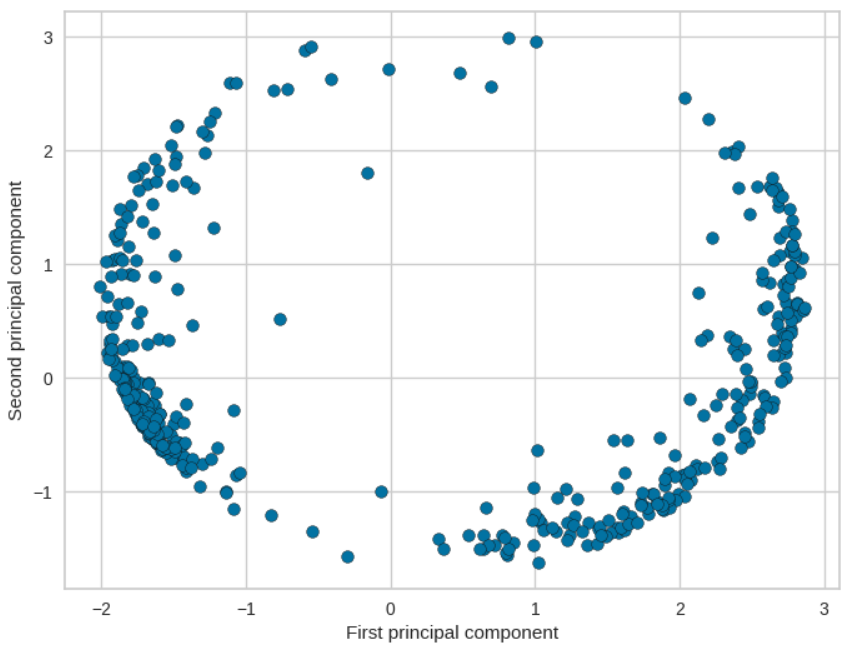
\includegraphics[width=\textwidth]{images/pca.png}
		\caption{PCA Visualization of Gene Expression Profiles During Sporulation}
		\label{fig:pca}
	\end{minipage}\hfill
	\begin{minipage}{0.45\textwidth}
		\centering
		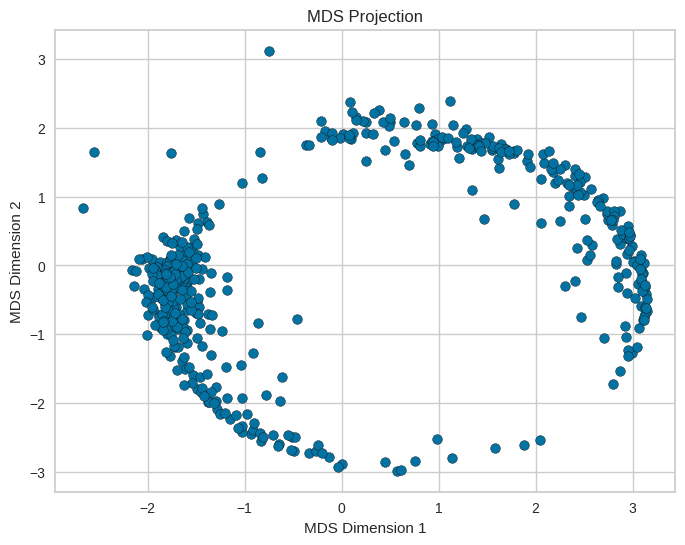
\includegraphics[width=\textwidth]{images/mds.png}
		\caption{MDS Visualization of Gene Expression Profiles During Sporulation}
		\label{fig:mds}
	\end{minipage}
\end{figure}
The resulting two principal components are visualized in figure \ref{fig:pca} using a scatter plot, where the x-axis represents the first principal component and the y-axis represents the second principal component. This visualization allows for a clearer understanding of the data's structure, revealing potential clusters and relationships among gene expression profiles during the sporulation process. Overall, PCA facilitates a more straightforward interpretation of complex datasets, making it easier to analyze patterns in gene expression.
\\

Similar to PCA, the resulting visualization in figure \ref{fig:mds} provides valuable insights into the relationship between samples, allowing for the identification of patterns and potential clustering of gene expression profiles during sporulation. Both techniques, PCA and MDS, are complementary and can provide similar information about the underlying structure of the data, assisting in the interpretation of results and the identification of relationships between variables.

\subsection{First aproach to clustering}

To further explore the relationships within the gene expression data, we apply K-means clustering using the MDS-reduced dimensions. Based on the results from the elbow method, we choose k=4 as the optimal number of clusters. The following code snippet demonstrates the implementation of MDS followed by K-means clustering:

\begin{lstlisting}[style=mypython, label=fig:pca_code,caption=Clustering using MDS and k-Means]
	
	from sklearn.manifold import MDS
	from sklearn.cluster import KMeans
	import matplotlib.pyplot as plt
	
	# Apply MDS to reduce dimensionality
	mds = MDS(n_components=2, random_state=42)
	x_mds = mds.fit_transform(x)
	
	# Perform clustering with K-means
	clusterer = KMeans(n_clusters=4, random_state=42)
	cluster_labels = clusterer.fit_predict(x_mds)
	
	# Visualize the formed clusters
	plt.figure(figsize=(8, 6))
	plt.clf()
	plt.scatter(x_mds[:, 0], x_mds[:, 1], c=cluster_labels, edgecolor="k", cmap=plt.cm.Set1)
	
	# Obtain the centers of the clusters
	centers = clusterer.cluster_centers_
	
	# Draw red circles at the centers of the clusters
	plt.scatter(centers[:, 0], centers[:, 1], marker="o", c="red", s=200, edgecolor="k")
	
	plt.xlabel("MDS Dimension 1")
	plt.ylabel("MDS Dimension 2")
	plt.title("K-means Clustering on MDS Projection")
	plt.show()
	
\end{lstlisting}
The visualization (Figure \ref{fig:mds_k4}) illustrates the clusters formed by K-means, with different colors representing different clusters. Additionally, the red circles indicate the centers of the clusters, providing insight into the central tendencies of the identified groups. This approach allows for a clearer understanding of how gene expression profiles are organized and related during the sporulation process.
\begin{figure}[H]
	\centering
	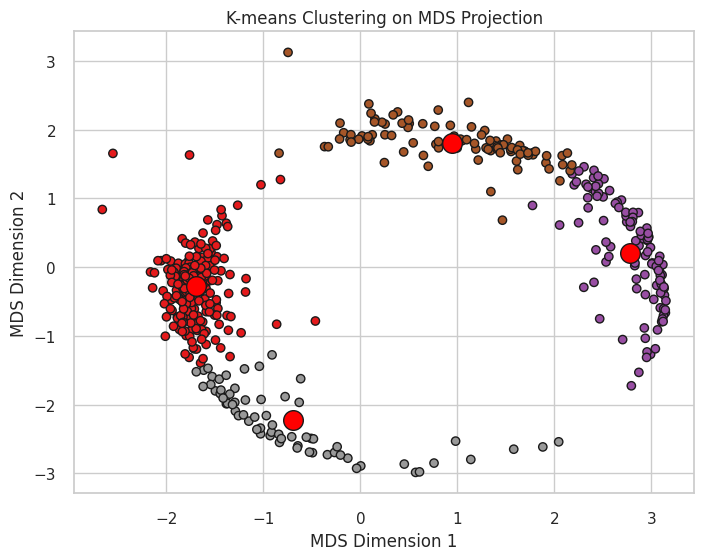
\includegraphics[width=.6\textwidth]{images/mds_k4.png}
	\caption{Visualization of clustering k=4}
	\label{fig:mds_k4}
\end{figure}

Moreover, each cluster is represented against the time variables \ref{lst:violin} to gain a better understanding of how these gene clusters are expressed at different time points.

Violin plots effectively illustrate the distribution of each variable, enabling us to observe variations in central tendency and spread across clusters. This visualization is particularly valuable for interpreting how the characteristics of gene expression profiles differ in relation to the identified clusters over time.

\begin{lstlisting}[style=mypython, caption=Violin Plots of Variables by Cluster, label=lst:violin]
	import math
	# Number of variables to plot
	num_vars = len(df.columns[1:-1])
	
	# Calculate rows and columns for the subplots
	cols = 3  # Number of plots per row
	rows = math.ceil(num_vars / cols)  # Number of rows needed
	
	# Create subplots
	fig, axes = plt.subplots(rows, cols, figsize=(cols * 6, rows * 4))
	fig.tight_layout(pad=5.0)  # Spacing between plots
	
	# Iterate over the variables and plot them
	for i, var in enumerate(df.columns[0:-1]):
		row = i // cols
		col = i % cols
		sns.violinplot(x=df['cluster'], y=var, data=df, ax=axes[row, col])
		axes[row, col].set_title(f'Violin Plot for {var} by Cluster')
	
	# Remove empty axes if there are any
	for i in range(num_vars, rows * cols):
		fig.delaxes(axes.flat[i])
	
	plt.show()
\end{lstlisting}

\begin{figure}[H]
	\centering
	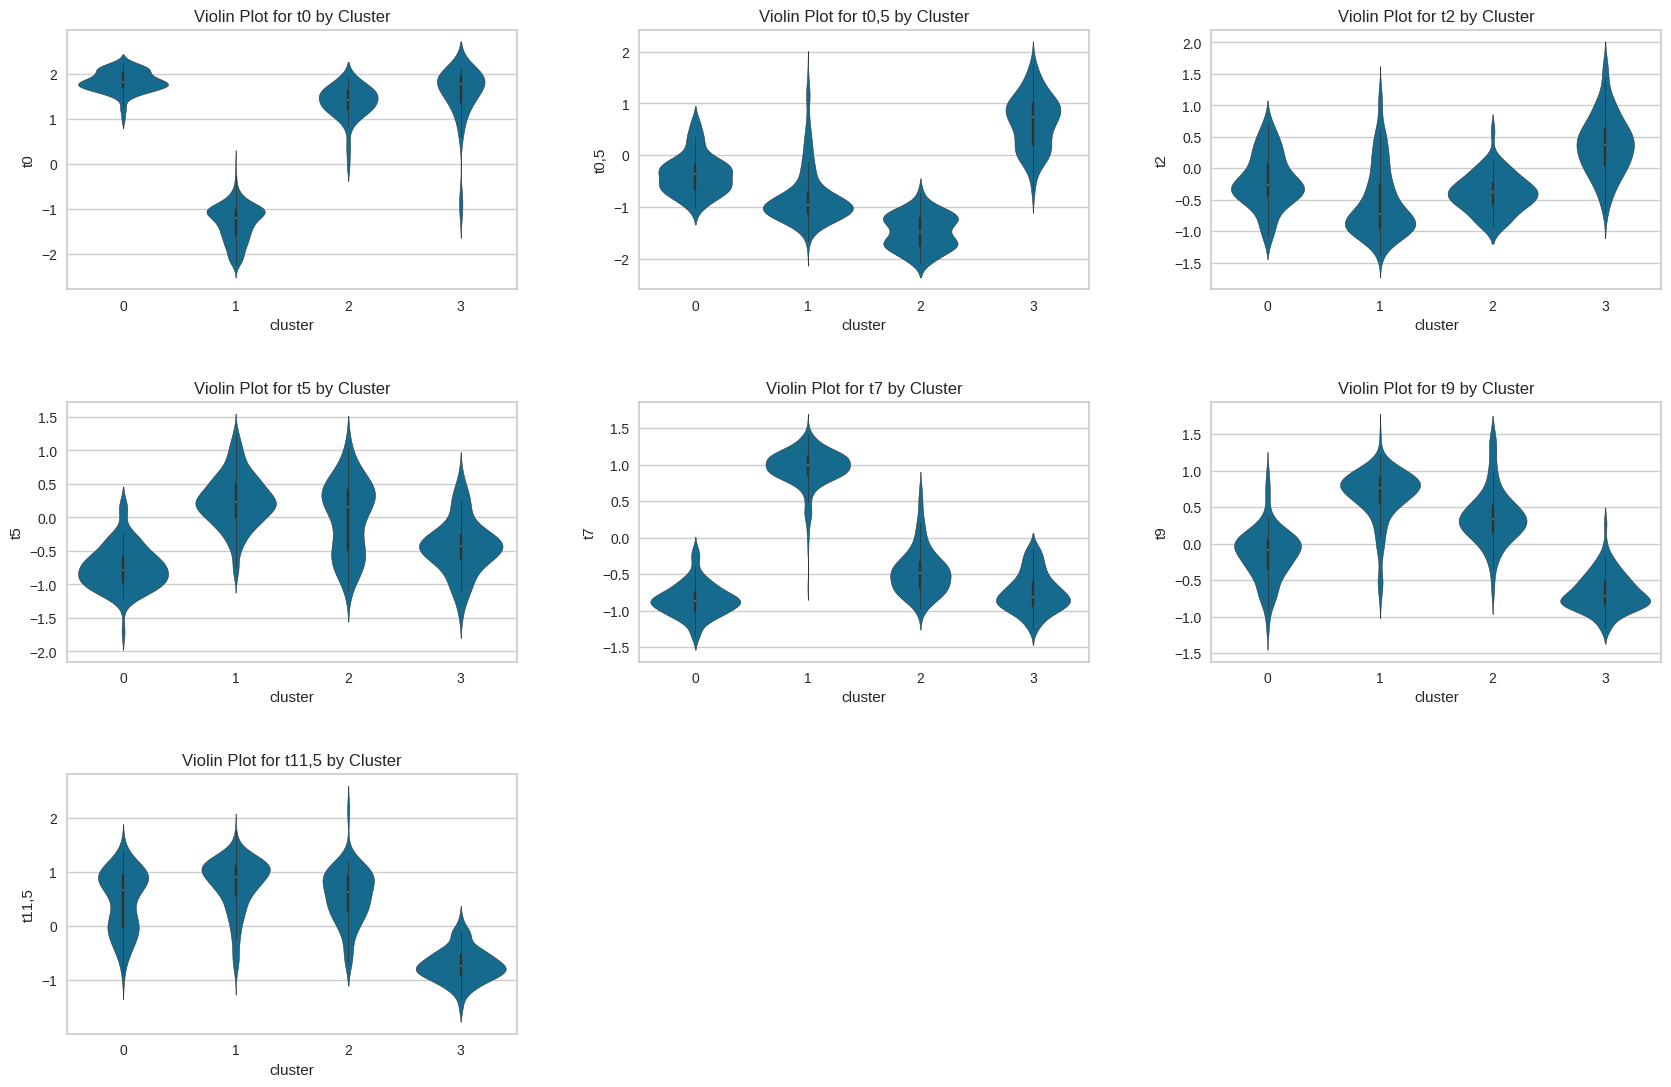
\includegraphics[width=\textwidth]{images/violin.png}
	\caption{Violin Plots of Variables by Cluster}
	\label{fig:violin_plots}
\end{figure}

In the Figure \ref{fig:violin_plots}, it is observed that some gene clusters are expressed coordinately at nearly every time point. This may indicate that these genes belong to the same functional group. Therefore, as seen in the MDS analysis, they might be incorrectly grouped. 

\subsection{Clustering comparation}

In this section, we compare various clustering methods (k-means, agglomerative clustering, and Gaussian mixture models) along with different numbers of clusters. This comparison employs multiple validation techniques to provide a comprehensive understanding of how well these clustering methods perform on the dataset. 

\begin{lstlisting}[style=mypython, caption=Clustering Metrics Across Different Methods, label=lst:violin]
# Iterate over different methods and values of k
for method_name, method in methods.items():
	for k in range(2, 15):  # Start at 2 so that the Silhouette score makes sense
		if method_name == 'KMeans':
			clusterer = method(n_clusters=k, random_state=42)
			cluster_labels = clusterer.fit_predict(x)
			centroids = clusterer.cluster_centers_
		elif method_name == 'Agglomerative':
			clusterer = method(n_clusters=k)
			cluster_labels = clusterer.fit_predict(x)
			centroids = None  # Agglomerative does not have centroids
		elif method_name == 'Gaussian Mixture':
	_state=42)
			cluster_labels = clusterer.fit_predict(x)
			centroids = clusterer.means_
			
		# Silhouette Score
		silhouette_avg = silhouette_score(x, cluster_labels)
		
		# Mean Distance to Centroids (solo para metodos con centros)
		if centroids is not None:
			mean_distance = np.mean(np.min(cdist(x, centroids), axis=1))
		else:
			mean_distance = np.nan
		
		# Average Distance Between Clusters
		avg_distance = 0
		for i in range(k):
			for j in range(i + 1, k):
				avg_distance += np.mean(cdist(x[cluster_labels == i], x[cluster_labels == j]))
				avg_distance /= (k * (k - 1)) / 2  # Overall average
		
		# Non-O	clusterer = method(n_components=k, randomverlap Measure
		non_overlap = non_overlap_measure(cluster_labels)

\end{lstlisting}

\begin{figure}[H]
	\centering
	\begin{minipage}{0.45\textwidth}
		\centering
		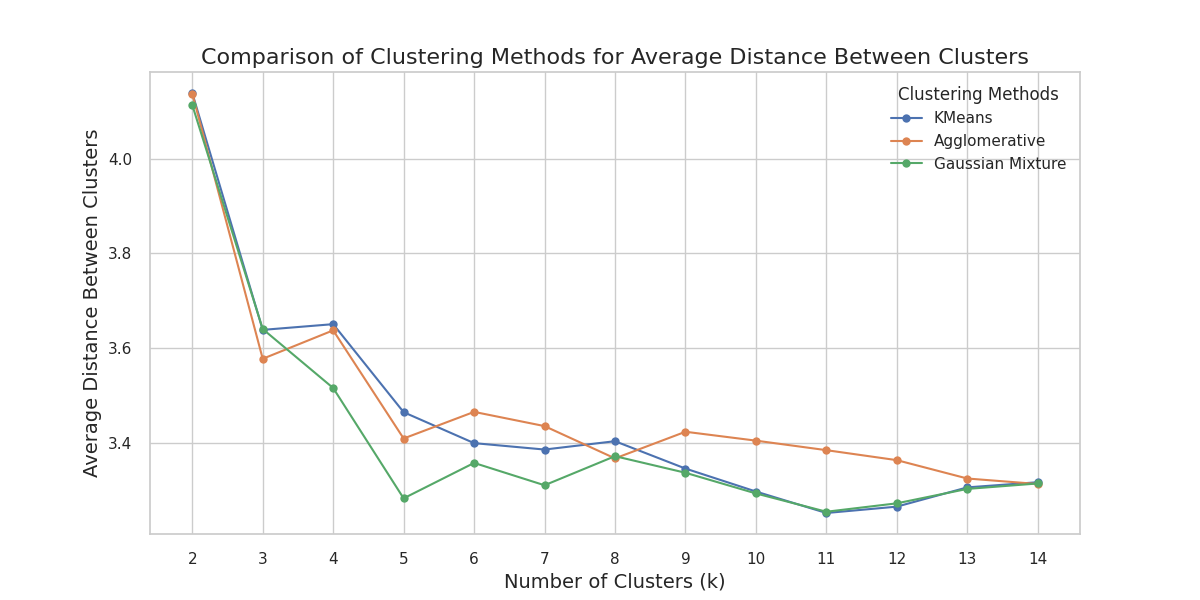
\includegraphics[width=\textwidth]{images/clustering_Average Distance Between Clusters.png}
		\caption{Average Distance Between Clusters}
		\label{fig:average_distance}
	\end{minipage}\hfill
	\begin{minipage}{0.45\textwidth}
		\centering
		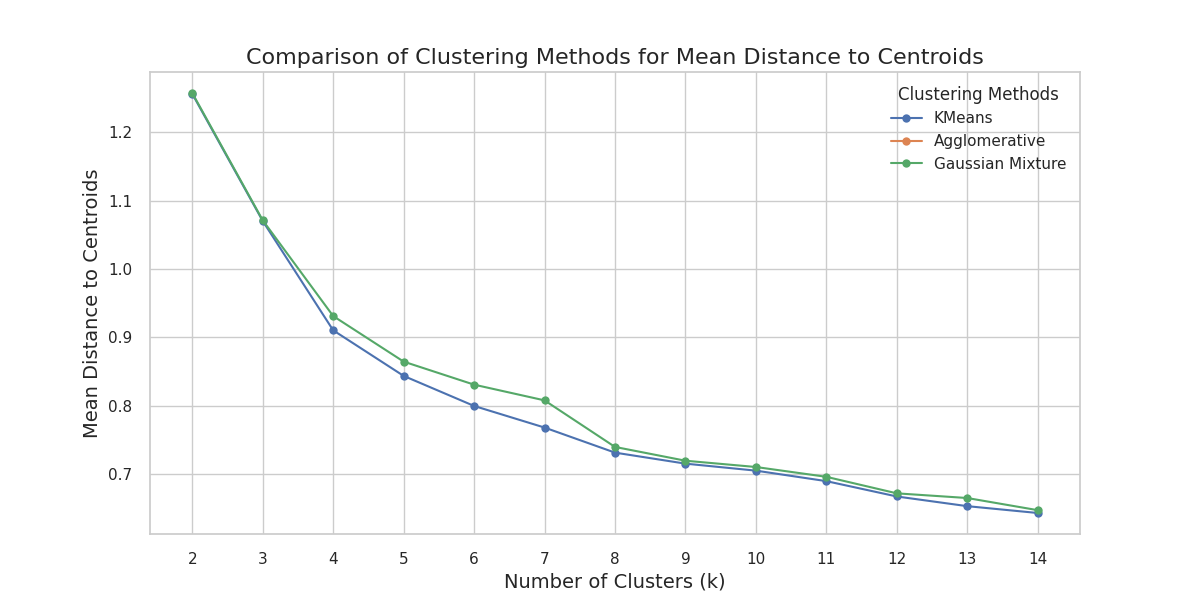
\includegraphics[width=\textwidth]{images/clustering_Mean Distance to Centroids.png}
		\caption{Mean Distance to Centroids}
		\label{fig:mean_distance}
	\end{minipage}
	
	\vspace{0.5cm} % Espacio vertical entre filas
	
	\begin{minipage}{0.45\textwidth}
		\centering
		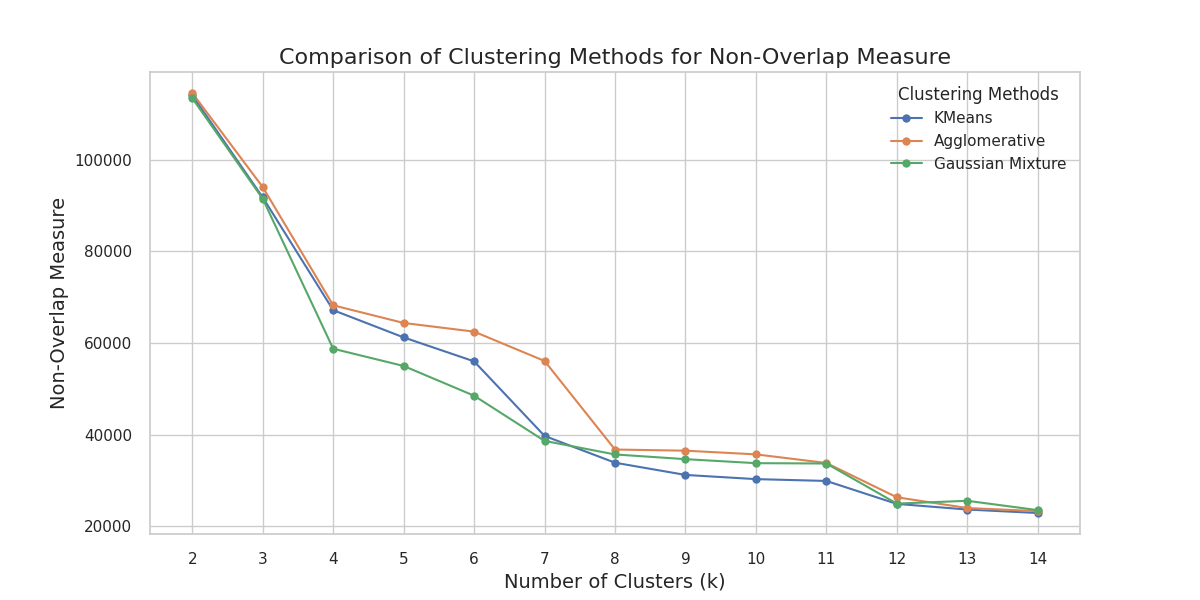
\includegraphics[width=\textwidth]{images/clustering_Non-Overlap Measure.png}
		\caption{Non-Overlap Measure}
		\label{fig:non_overlap}
	\end{minipage}\hfill
	\begin{minipage}{0.45\textwidth}
		\centering
		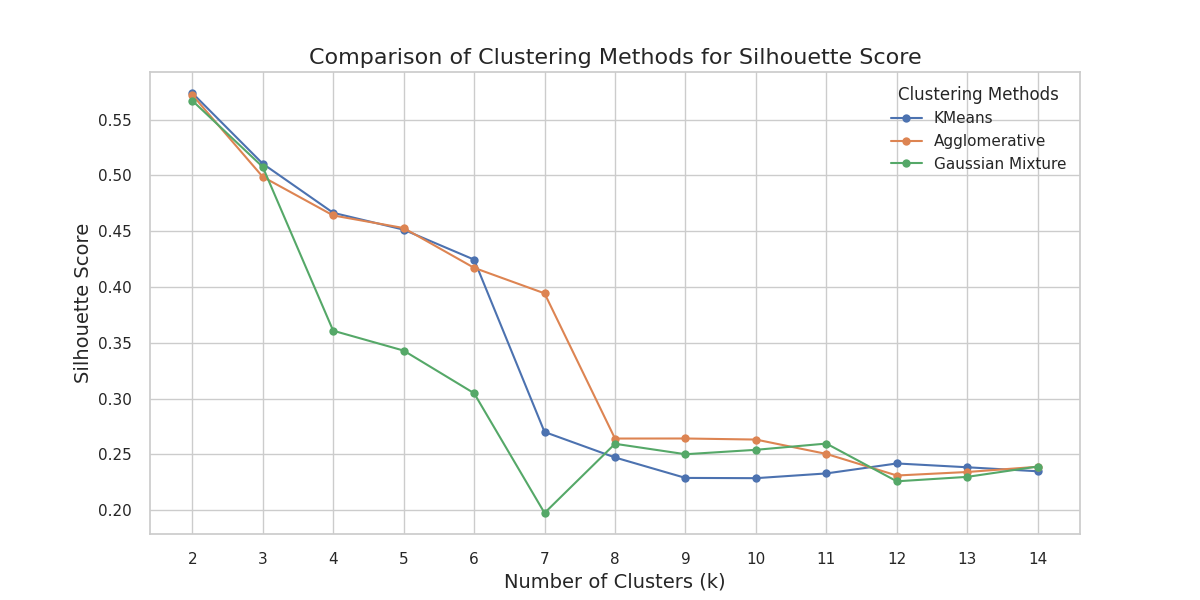
\includegraphics[width=\textwidth]{images/clustering_Silhouette Score.png}
		\caption{Silhouette Score}
		\label{fig:silhouette_score}
	\end{minipage}
	
	\caption{Comparison of Clustering Methods}
	\label{fig:clustering_methods}
\end{figure}

After comparing the K-means, Gaussian Mixture, and Agglomerative Clustering methods, we observed that in all cases, the most appropriate number of clusters is k=2. The average distance between clusters was slightly better in our results, particularly at k=2, indicating better-defined cluster separation. Similarly, the mean distance to centroids also showed improved performance at k=2 in our analysis, further supporting that this value provides the most accurate and cohesive clustering solution for our data across all methods evaluated.
 
\subsection{Silhouettes}
To enhance our understanding of the clustering results, we will employ silhouette analysis, a technique that evaluates the quality of clustering solutions by measuring how similar an object is to its own cluster compared to other clusters \cite{rousseeuw1987silhouettes}. Each data point's silhouette value is derived from two distances: the average distance to points in its own cluster (\(a(i)\)) and the average distance to points in the nearest neighboring cluster (\(b(i)\)). The silhouette score \(s(i)\) ranges from -1 to +1, where a score close to +1 indicates well-clustered points, a score near 0 suggests points on the border between clusters, and a score close to -1 indicates misclassified points. 
\\

Since the results obtained using the previous methods do not fully align with the findings reported in the literature, we will now apply the silhouette method to analyze our data. This approach will allow us to evaluate the consistency and quality of our clustering results in a more robust manner. By using the silhouette method, we aim to gain deeper insights into how well-separated our clusters are, as this metric considers both the cohesion within clusters and the separation between different clusters. This analysis should help us better understand the discrepancies between our findings and those reported in the original article, providing a more thorough validation of our results.

\begin{lstlisting}[style=mypython, label=fig:pca_code, caption=Implementation of Silhouette Analysis for Clustering Evaluation]
	import numpy as np
	import matplotlib.pyplot as plt
	from sklearn.cluster import KMeans
	from sklearn.metrics import silhouette_samples, silhouette_score
	
	# Create a range of k values
	range_k = range(2, 11)
	
	for k in range_k:
		# Create the KMeans model with the number of clusters k
		kmeans = KMeans(n_clusters=k, random_state=10)
		cluster_labels = kmeans.fit_predict(x)
	
		# If k is 1, the silhouette score cannot be calculated
		if k == 1:
		print(f"K = {k}: The silhouette score is not applicable.")
		continue
		
		# Calculate the average silhouette score for all points
		silhouette_avg = silhouette_score(x, cluster_labels)
		print(f"K = {k}: Average silhouette score = {silhouette_avg:.3f}")
		
		# Calculate the silhouette values for each point
		sample_silhouette_values = silhouette_samples(x, cluster_labels)
		
		# Create the silhouette plot
		fig, ax1 = plt.subplots(1, 1)
		fig.set_size_inches(7, 5)
		
		y_lower = 10
		for i in range(k):
			# Aggregate silhouette values for the clusters in order
			ith_cluster_silhouette_values = sample_silhouette_values[cluster_labels == i]
			ith_cluster_silhouette_values.sort()
			
			size_cluster_i = ith_cluster_silhouette_values.shape[0]
			y_upper = y_lower + size_cluster_i
		
			ax1.fill_betweenx(np.arange(y_lower, y_upper),
			0, ith_cluster_silhouette_values)
			
			y_lower = y_upper + 10  # Space between clusters
		
		# Draw the line for the average silhouette score
		ax1.axvline(x=silhouette_avg, color="red", linestyle="--")
		
		ax1.set_title(f"Silhouette plot for k = {k}")
		ax1.set_xlabel("Silhouette coefficient")
		ax1.set_ylabel("Cluster label")
		
		plt.show()
\end{lstlisting}


\begin{figure}[H]
	\centering
	\begin{minipage}{0.45\textwidth}
		\centering
		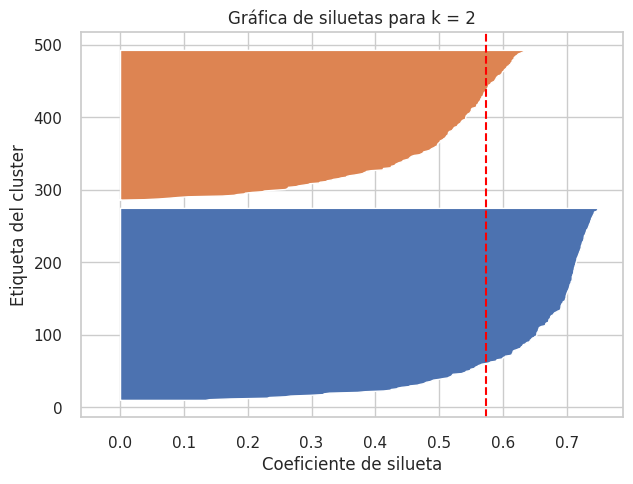
\includegraphics[width=\textwidth]{images/sil_2.png}
		\caption{Silhouette Score k=2, average: 0.57}
		\label{fig:sil2}
	\end{minipage}\hfill
	\begin{minipage}{0.45\textwidth}
		\centering
		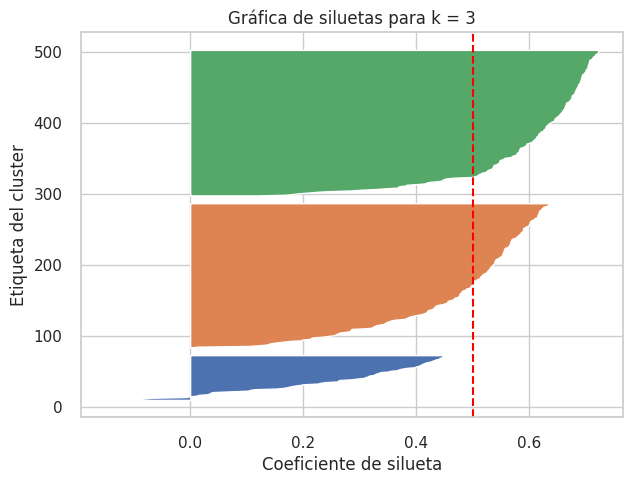
\includegraphics[width=\textwidth]{images/sil_3.png}
		\caption{Silhouette Score k=3, average: 0.5}
		\label{fig:sil3}
	\end{minipage}
	
	\vspace{0.5cm} % Espacio vertical entre filas
	
	\begin{minipage}{0.45\textwidth}
		\centering
		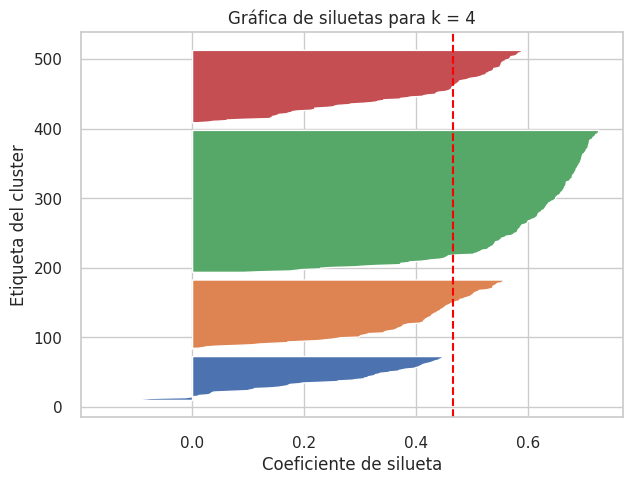
\includegraphics[width=\textwidth]{images/sil_4.png}
		\caption{Silhouette Score k=4, average: 0.46}
		\label{fig:sil4}
	\end{minipage}\hfill
	\begin{minipage}{0.45\textwidth}
		\centering
		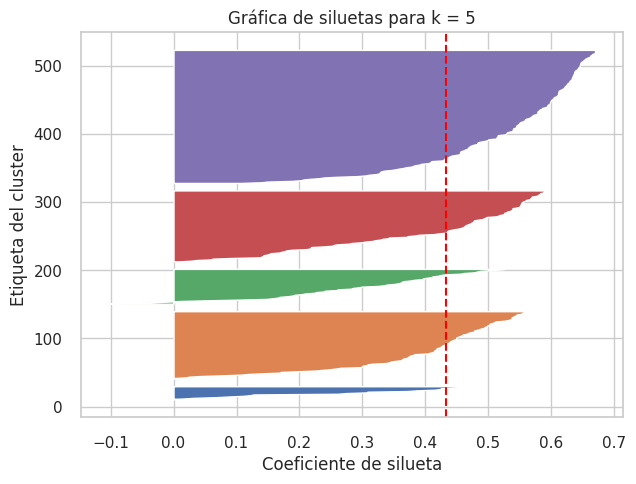
\includegraphics[width=\textwidth]{images/sil_5.png}
		\caption{Silhouette Score k=5, average: 0.43}
		\label{fig:sil5}
	\end{minipage}
	
	\caption{Comparison of silhouettes}
	\label{fig:clustering_methods}
\end{figure}
Once again, the results obtained reinforce the previous findings. This consistency across the analyses strengthens our confidence in the validity of our conclusions and highlights the robustness of our clustering approach. The alignment of results across different methods further emphasizes the reliability of our chosen clustering solution for our dataset.




\section{Conclusion}
The results we obtained suggest that the optimal value of k for our dataset is k=2. However, this finding contrasts with the conclusions drawn in previous studies, where k=7 is consistently reported as the most appropriate value. This discrepancy might be explained by the fact that our dataset and experimental conditions differ from those used in the literature. 
The study likely achieves its results by relying on external data sources that support the notion of classifying the data into seven distinct groups. This external validation may lead the researchers to aim for a clustering solution that aligns with this predetermined value. Furthermore, considering that the paper is over 22 years old, it is possible that the methodologies and datasets used may not reflect current standards or advancements in clustering techniques, which could contribute to the observed differences in outcomes between their findings and our analysis.
\\

Despite this divergence, the evidence strongly suggests that k=2 is the most suitable choice for our data, considering the information at our disposal. This conclusion is substantiated by several factors, including the results from principal component analysis (PCA) and multidimensional scaling (MDS) visualizations, which clearly indicate a natural grouping around two clusters. Additionally, the metrics obtained for all clusters further reinforce this finding, particularly when evaluating clustering quality through methods such as silhouette analysis, which consistently points to k=2 as the most appropriate value for our dataset.


\section{Repository Access}

All additional information, including the source code and full documentation of this project, is available in the GitHub repository \cite{silva2024github}.


% Incluir la bibliografía
\bibliographystyle{plain}  % Estilo de la bibliografía (por ejemplo, plain, alpha, ieee, etc.)
\bibliography{bibli}  % Nombre del archivo .bib sin la extensión

\end{document}
